\section{Zweierkomplement}

\begin{frame}{Ein asymmetrischer Zahlenbereich}
	\[
	\K_{\ell} = \{ x\in \Z \mid -2^{\ell-1} \leq x \leq 2^{\ell-1} -1 \} \;.
	\]
	\\[0.2cm]
	
	\begin{figure}
		\centering
		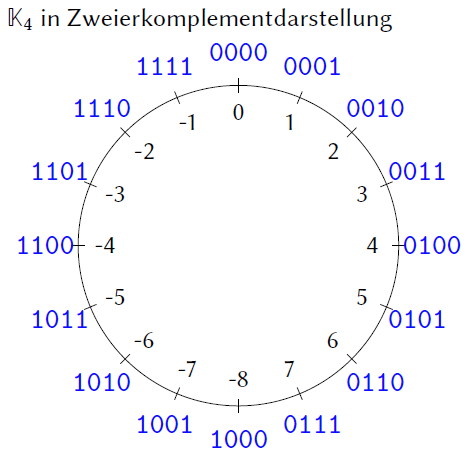
\includegraphics[scale=0.45]{ZK_K4}
	\end{figure}
	
\end{frame}

\begin{frame}{Zweierkomplement (ZK)}
	
	Ermöglicht Binärdarstellung positiver \textbf{und} negativer Zahlen. \\
	Besonders hardwareverträglich verglichen mit anderen Darstellungen \textit{(mehr dazu in Technischer Informatik)}.

	\begin{block}{Definition}
		Wollen Zweierkomplement der Länge $\ell$. \\ Haben $\fbin_\ell$: einfache Konvertierung nach Binär mit Länge $\ell$.
		$$\fZkpl_\ell(x) = \begin{cases} \word 0 \fbin_{\ell-1}(x), & \text{falls } x \geq 0 \\ 
										 \word 1 \fbin_{\ell-1}(2^{\ell-1}+x) & \text{falls } x < 0\end{cases}$$
		
		Äquivalent:
		$$\fZkpl_\ell(x) = \begin{cases} \fbin_{\ell}(x), & \text{falls } x \geq 0 \\ 
										 \fbin_{\ell}(2^{\ell}+x) & \text{falls } x < 0\end{cases}$$
	\end{block}
\end{frame}

\begin{frame}{ZK ausrechnen}
	$x \geq 0$: geschenkt \smiley \\
	$x < 0$:
	\begin{enumerate}
		\item Binärdarstellung von $\abs{x}$ berechnen
		\item Vorne mit Nullen auffüllen bis zur Länge $\ell$
		\item Alle binären Ziffern negieren
		\item 1 addieren
	\end{enumerate}
	
	\begin{Beispiel}
		 $$\fZkpl_4(-2): 2 \stackrel{\fRepr_2}{\?>} \word{10} \stackrel{\text{Nullen}}{\?>} \word{0010} \stackrel{\text{negieren}}{\?>} \word{1101} \stackrel{+1}{\?>} \underline{\word{1110}}. $$
		 Achtung, das ist \textbf{keine offizielle Schreibweise!} Das will ich auf'm Übungsblatt nicht sehen!
	\end{Beispiel}
\end{frame}

\begin{frame}{ZK ausrechnen}
	\begin{Beispiel}
		\begin{align*}
		\fZkpl_5(0)  &= \visible<2->{\word{00000}} \\
		\fZkpl_5(2) &= \visible<3->{\word{00010}} \\
		\fZkpl_5(15) &= \visible<4->{\word{01111}} \\
		\fZkpl_5(-1) &= \visible<5->{\word{11111}} \\
		\fZkpl_5(-6) &= \visible<6->{\word{11010}} \\
		\fZkpl_5(-16) &= \visible<7->{\word{10000}}
		\end{align*}
	\end{Beispiel}
\end{frame}

\begin{frame}{ZK ausrechnen -- formal}
	Die einzelnen Schritte können wir auch formal angeben:\\
	(Wir operieren jeweils auf Wörtern aus $\{\word 0, \word 1\}^* = Z_2^*$) \\[0.5em]
	1. Binärdarstellung von $\abs{x}$ berechnen: $Repr_2(\abs{x})$ \\
	2. Vorne mit Nullen auffüllen bis zur Länge $\ell$\\ \pause
	\begin{threealign}
		Fill_\ell : Z_2^m &\functionto& Z_2^\ell \qquad (m \le \ell) \\ \visible<3-> {
		w &\mapsto& \begin{cases}
		\word 0^\ell, & w = \varepsilon \\
		Fill_{\ell-1}(w') \cdot \mu, & w = w' \cdot \mu \text{ mit } w' \in Z_2^*, \mu \in Z_2
		\end{cases} \\
		\text{Oder viiieeel einfacher: }& \\
		w &\mapsto& \begin{cases}
		w, & \setsize{w} = \ell \\
		Fill_\ell(\word 0 w), & \text{sonst}
		\end{cases} \\
	}
	\end{threealign}
	\pause[4] 3. / 4. Analog %TODO
\end{frame}